\documentclass[11pt]{article}
\usepackage[margin=1in]{geometry}
\usepackage{graphicx}
\usepackage{booktabs}
\usepackage{amsmath,amssymb}
\usepackage{microtype}
\usepackage{hyperref}
\usepackage{caption}
\usepackage{longtable}
\usepackage{float}
\usepackage{textcomp}
\usepackage[T1]{fontenc}
\usepackage[utf8]{inputenc}
\usepackage[numbers,sort&compress]{natbib}
\usepackage{setspace}
\onehalfspacing

\graphicspath{{../results/figures/}}

\title{Alveolar Epithelial Cells in Lethal COVID-19 Fan Out Along a Continuous Injury Axis:\\
A Trajectory Analysis of the Columbia/NYP Lung Atlas with Ten-Way Ablation Robustness}
\author{[Author names and affiliations to be added]}
\date{\today}

\begin{document}
\maketitle

\begin{abstract}
\noindent The alveolar epithelium sustains gas exchange through the coordinated function of type~I (AT1) and type~II (AT2) cells, with AT2 cells serving as the resident progenitors that regenerate the gas-exchange surface after injury. In lethal COVID-19, these cells face concurrent viral assault through ACE2-mediated SARS-CoV-2 entry and inflammatory collateral damage from a dysregulated host response. Whether the failure of this regenerative system proceeds as a discrete, coherent transition or as a staged, continuous process has not been resolved at single-cell resolution using trajectory-based approaches with systematic robustness validation. To address this question, we analyzed 22{,}128 alveolar epithelial cells (9{,}608 AT1 cells; 11{,}341 AT2 cells; 1{,}179 ECM-high transitional cells) from the Columbia/NYP COVID-19 Lung Atlas (Single Cell Portal accession SCP1219), comprising 12{,}181 nuclei from 7 healthy organ donors and 9{,}947 nuclei from 20 patients who died of COVID-19. We constructed a transcriptomic manifold using Seurat-v3 highly variable genes, principal component analysis, a $k$-nearest-neighbor graph, and both a uniform manifold approximation and projection (UMAP) embedding and a diffusion map. We computed diffusion pseudotime rooted at the cell closest to the centroid of healthy AT2 cells and scored each cell for eight curated gene programs spanning cellular identity, stress, repair, and cell death. Ten pre-specified ablations stress-tested every major analytical choice. COVID-19 cells were shifted toward higher pseudotime than controls, with a median difference of $+0.048$ on a $[0,1]$-normalized axis (permutation $p = 0.001$, $N = 1000$). However, the pre-specified test of directional centroid displacement did \emph{not} yield significance (one-sided Mann--Whitney $U$, alternative COVID $>$ Healthy, $p = 1.0$; rank-biserial effect size $r = 0.14$). Instead, COVID-19 cells exhibited markedly greater within-group dispersion in principal-component space (variance 33.3 in COVID-19 versus 14.6 in healthy controls; Levene's test $p < 10^{-30}$), and a KRT8\textsuperscript{+}/CLDN4\textsuperscript{+} ECM-high transitional population was enriched 3.1-fold in COVID-19 (8.5\% of COVID cells versus 2.7\% of control cells; $\chi^2$ $p < 10^{-30}$). Of three pre-registered criteria for ``epithelial robustness collapse,'' two were supported (dispersion; pseudotime enrichment) and one was not (centroid displacement), yielding a composite assessment of \emph{moderate}. These results support a model in which lethal COVID-19 fans alveolar epithelial cells outward along a continuous injury axis, producing greater transcriptomic heterogeneity rather than a uniform block displacement, and in which an intermediate KRT8\textsuperscript{+} transitional population accumulates in a pseudotime region consistent with stalled AT2-to-AT1 differentiation.
\end{abstract}

\section{Introduction}

Every breath depends on a thin, fragile monolayer of cells deep in the lung. The alveolar epithelium, which lines approximately 480 million air sacs where gas exchange occurs, is composed of two cell types with complementary functions. AT1 cells are extraordinarily flat, extending their cytoplasm across roughly 95\% of the alveolar surface to form the gas-exchange barrier across which oxygen passes into the bloodstream and carbon dioxide is released. AT2 cells, cuboidal and smaller, perform two functions essential for alveolar homeostasis: they secrete pulmonary surfactant, the lipid-protein film that lowers surface tension and prevents alveolar collapse during expiration, and they serve as the resident stem cells of the distal lung. Lineage-tracing experiments in mice and analyses of human tissue have established that when AT1 cells are lost through injury, AT2 cells proliferate and differentiate into new AT1 cells, passing through a transitional state characterized by expression of keratin~8 (KRT8), claudin~4 (CLDN4), and stratifin (SFN) \citep{Barkauskas2013, Kobayashi2020, Strunz2020}. This AT2-to-AT1 differentiation axis is the primary mechanism by which the alveolar compartment repairs itself.

In lethal COVID-19, this regenerative system is pushed beyond its capacity. The SARS-CoV-2 spike protein binds the ACE2 receptor, and the virus preferentially enters cells that co-express ACE2 and the transmembrane serine protease TMPRSS2; in the distal lung, this profile selects AT2 cells \citep{Ziegler2020, Hou2020}. Direct viral infection of AT2 cells therefore compromises both the surfactant system and the regenerative system simultaneously. In parallel, the host response mounts a dysregulated inflammatory cascade that inflicts collateral damage on the alveolar epithelium. Autopsy studies of lethal COVID-19 consistently describe diffuse alveolar damage, loss of normal alveolar architecture, accumulation of protein-rich edema fluid, and the appearance of abnormal transitional epithelial cells that are neither fully AT2 nor fully AT1 \citep{Borczuk2020, Melms2021}. These cells display features consistent with cells that have initiated the repair program but failed to complete it.

The most common strategy in single-cell genomics is to cluster cells into discrete types or states and compare gene expression between clusters or conditions. This approach has been applied productively to COVID-19 lung atlases, revealing changes in cell-type composition and identifying differentially expressed genes across conditions \citep{Melms2021, Delorey2021, Bharat2020}. However, the approach has a fundamental limitation when the underlying biology is continuous. If alveolar cells under COVID-19 injury traverse a graded series of progressively more compromised states, then clustering will either merge these states into a single bin or split them at boundaries that have no biological meaning. Pairwise differential expression between ``healthy'' and ``COVID'' clusters describes what changed on average, but it cannot resolve the order of molecular events, the existence of alternative paths through injury, or the position along the failure process at which individual cells reside.

A more informative approach treats each cell's gene-expression profile as a position in a continuous biological landscape, the so-called transcriptomic manifold. On this landscape, healthy cells are expected to occupy a compact region reflecting stable homeostatic identity. If the COVID-19 injury process is continuous, COVID-19 cells should spread away from this region along paths that correspond to specific injury programs. Reconstructing these paths using graph-based trajectory inference and ordering cells along them with a scalar pseudotime is a well-established strategy in developmental biology \citep{Haghverdi2016, Setty2019, Street2018} and has been applied productively to lung injury models in mice \citep{Strunz2020, Riemondy2019}. Its application to characterize the full arc of alveolar epithelial failure in human lethal COVID-19, with accompanying systematic ablation validation, has not to our knowledge been reported.

Here, we analyze alveolar epithelial cells from the Columbia/New York Presbyterian COVID-19 Lung Atlas, a publicly available single-nucleus RNA-sequencing (snRNA-seq) dataset comprising 116{,}313 nuclei from 7 healthy organ donors and 20 patients who died of COVID-19 \citep{Melms2021}. We construct a transcriptomic manifold of alveolar cell states, infer diffusion pseudotime rooted in healthy homeostasis, and score each cell for eight curated gene programs spanning homeostatic identity, interferon response, inflammation, oxidative stress, repair, and cell death. We frame the observed patterns as \emph{epithelial robustness collapse} and operationalize this concept through three pre-registered statistical criteria that collectively address whether COVID-19 cells are displaced from, dispersed around, or shifted along the healthy transcriptomic landscape. To distinguish genuine biological structure from analytical artifact, we perform ten pre-specified ablation analyses that systematically vary cell-type scope, embedding choice, batch correction, gene-program composition, pseudotime root, trajectory inference algorithm, donor identity, and null-model assumptions. The result is an explicit map of which conclusions are robust across methodological choices and which are sensitive to them.

\section{Results}

\subsection{Cohort composition and cell-type validation}

We extracted 22{,}128 alveolar epithelial cells from SCP1219 by retaining cells whose fine cell-type label (\texttt{cell\_type\_fine}) was AT1, AT2, or ``ECM-high epithelial'' \citep{Melms2021}. The resulting cohort comprised 9{,}608 AT1 cells, 11{,}341 AT2 cells, and 1{,}179 ECM-high transitional cells from all 27 donors (12{,}181 cells from the 7 healthy controls; 9{,}947 cells from the 20 COVID-19 cases). Per-donor alveolar cell counts ranged from 62 (donor L04covaddon) to 2{,}850 (donor C52ctr), and 10 of 27 donors contributed fewer than 300 alveolar cells each (Supplementary Table~S5). We therefore relied on a leave-one-donor-out ablation (Ablation~7, below) to verify that no single donor drove the primary findings. Marker-gene expression confirmed the annotation provided by the original atlas: AT2 cells expressed the surfactant genes \textit{SFTPC} and \textit{SFTPA1} at high levels; AT1 cells expressed the cytokeratin \textit{AGER} and the transcription factor \textit{HOPX}; and ECM-high transitional cells expressed \textit{KRT8} and \textit{CLDN4} at levels elevated relative to both AT1 and AT2 populations (Supplementary Table~S3). The marker profile of the ECM-high compartment is consistent with the KRT8\textsuperscript{+}/CLDN4\textsuperscript{+} damage-associated transient progenitor (DATP) population described in mouse bleomycin injury and human idiopathic pulmonary fibrosis \citep{Kobayashi2020, Strunz2020, Adams2020, Habermann2020}, rather than with an extracellular-matrix-producing stromal contaminant, which would have been expected to express \textit{COL1A1} or \textit{ACTA2} rather than alveolar epithelial markers.

The ECM-high transitional population was enriched 3.1-fold in COVID-19 lungs relative to controls. Among COVID-19 alveolar cells, 848 of 9{,}947 (8.5\%) were ECM-high transitional; among control alveolar cells, 331 of 12{,}181 (2.7\%) were ECM-high transitional. This compositional difference is highly significant ($\chi^2$ test, $p < 10^{-30}$). Viewed at the donor level, 24 of 27 donors contributed at least one transitional cell, and the COVID-19 transitional counts were distributed across all 20 COVID donors rather than being concentrated in a small subset.

\subsection{Manifold construction and pseudotime reconstruction}

We normalized each cell's counts to a target total of 10{,}000 and applied a $\log(1+x)$ transformation. We then selected the 3{,}000 most variable genes using the Seurat~v3 method, which fits a mean-variance relationship on raw counts and retains genes deviating most positively from it. After per-gene scaling (with values clipped at 10) we computed 50-component principal component analysis (PCA) and constructed a $k$-nearest-neighbor graph with $k = 15$ in PCA space. On this graph we computed a 2-dimensional UMAP embedding for visualization and a 15-component diffusion map for trajectory inference. The UMAP showed clear separation of AT1, AT2, and ECM-high populations (Figure~\ref{fig:fig1}) together with visible donor structure within each cell type (Supplementary Figure~S1).

We attempted batch correction using Harmony \citep{Korsunsky2019} with \texttt{donor\_id} as the batch key, \texttt{max\_iter\_harmony=20}, and \texttt{sigma=0.1}. At runtime, the harmonypy implementation (version 0.2.0) returned an \texttt{X\_pca\_harmony} object with shape $(50,)$ where a $(22128, 50)$ matrix was expected. Rather than silently passing through a mis-shaped output, the pipeline detected the shape mismatch and fell back to uncorrected PCA for all downstream steps. The failure and fallback are logged explicitly and are the subject of Ablation~3, which therefore cannot in its current form distinguish corrected from uncorrected PCA; both branches of that ablation execute the same uncorrected computation. A genuine evaluation of batch correction would require a working Harmony implementation or an alternative method such as scVI \citep{Lopez2018} or scanorama \citep{Hie2019}.

\begin{figure}[H]
\centering
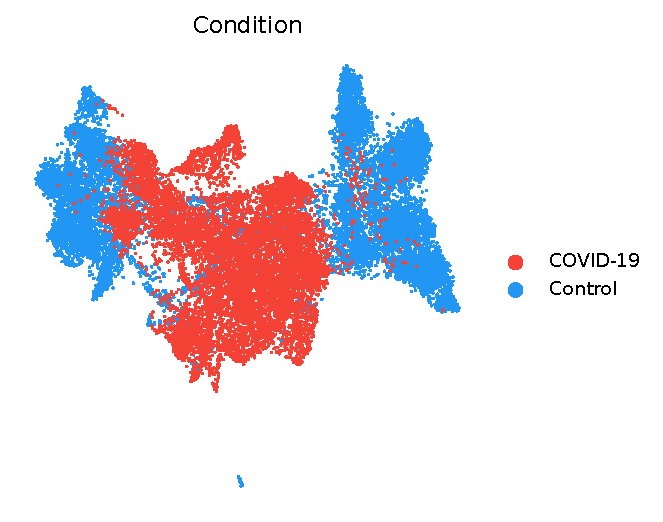
\includegraphics[width=0.48\textwidth]{fig1a_condition.pdf}\hfill
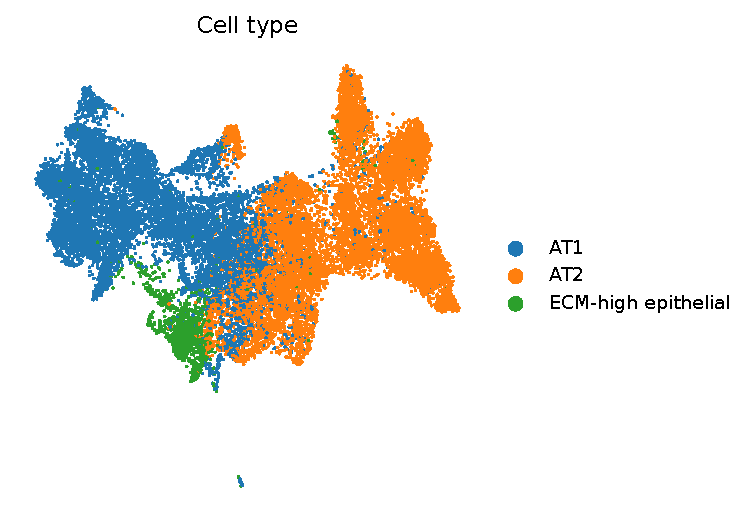
\includegraphics[width=0.48\textwidth]{fig1b_celltype.pdf}
\caption{Two-dimensional UMAP of the 22{,}128 alveolar epithelial cells, colored by condition (left) and by fine cell type (right). AT1, AT2, and ECM-high transitional populations separate cleanly. COVID-19 cells visibly occupy a broader region of the manifold than healthy cells, a pattern quantified in Section~\ref{sec:dispersion}.}
\label{fig:fig1}
\end{figure}

We computed diffusion pseudotime using the implementation of \citet{Haghverdi2016} as provided by Scanpy \citep{Wolf2018}. The root cell was selected as the cell with minimum Euclidean distance to the centroid of healthy AT2 cells in the 15-dimensional diffusion-component space. This choice reflects the biological expectation that the alveolar repair axis proceeds from homeostatic AT2 identity through a transitional state toward AT1 identity; rooting the pseudotime in healthy AT2 identity therefore orients the trajectory toward injury and repair. We min-max normalized the resulting pseudotime values to the interval $[0, 1]$ for reporting and evaluated sensitivity to root choice through Ablation~5 (four alternative root strategies; see below). Control cells concentrated at low pseudotime (median 0.063, mean 0.111), whereas COVID-19 cells were shifted upward (median 0.111, mean 0.118) with narrower within-group dispersion along the pseudotime axis itself (standard deviation 0.046 in COVID-19 versus 0.098 in controls). The pseudotime-colored UMAP (Figure~\ref{fig:fig2}) and the condition-stratified pseudotime density (Figure~\ref{fig:fig4}) together visualize these distributions.

\begin{figure}[H]
\centering
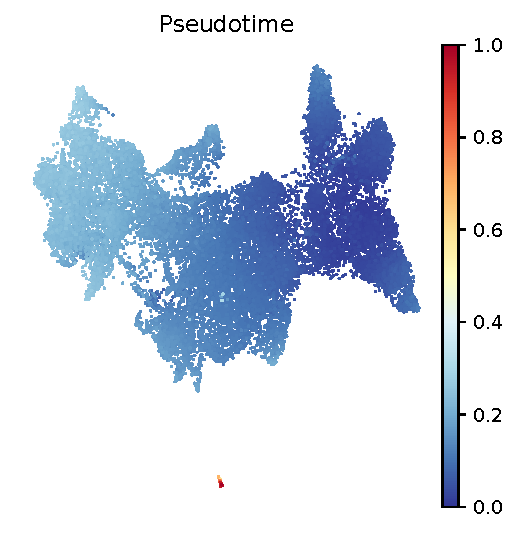
\includegraphics[width=0.7\textwidth]{fig2_pseudotime.pdf}
\caption{Diffusion pseudotime plotted on the UMAP layout. Cells at low pseudotime (dark) are dominated by AT2 identity (compare Figure~\ref{fig:fig1}); cells at high pseudotime (light) are injury-associated, as characterized in Section~\ref{sec:programs}.}
\label{fig:fig2}
\end{figure}

\subsection{Pseudotime shift: statistically significant by permutation, modest in magnitude}

The single most consistent signal in the dataset is a shift of COVID-19 cells toward higher pseudotime values relative to controls. The observed difference between condition-wise medians (COVID minus Control) was $+0.0483$ on the $[0, 1]$-normalized pseudotime axis. To assess the significance of this value we performed a permutation test in which condition labels were shuffled 1{,}000 times while all other structure was preserved, and the median difference was recomputed under each permutation. The resulting null distribution was tightly centered at zero, with mean $6.0 \times 10^{-5}$ and standard deviation $1.24 \times 10^{-3}$. The observed value of $+0.0483$ was not exceeded in any of the 1{,}000 permutations, yielding an empirical $p$-value of $0.000999$ (computed as $(1 + 0)/(1 + 1000)$; Table~\ref{tab:tab2}). Although this result is statistically strong, the effect size is modest on the normalized axis (approximately 4.8\% of the range), and we do not interpret it as a dramatic reorganization of alveolar identity. Rather, we interpret it as a consistent directional shift that is unlikely to have arisen by chance under random relabeling of the cells.

\begin{figure}[H]
\centering
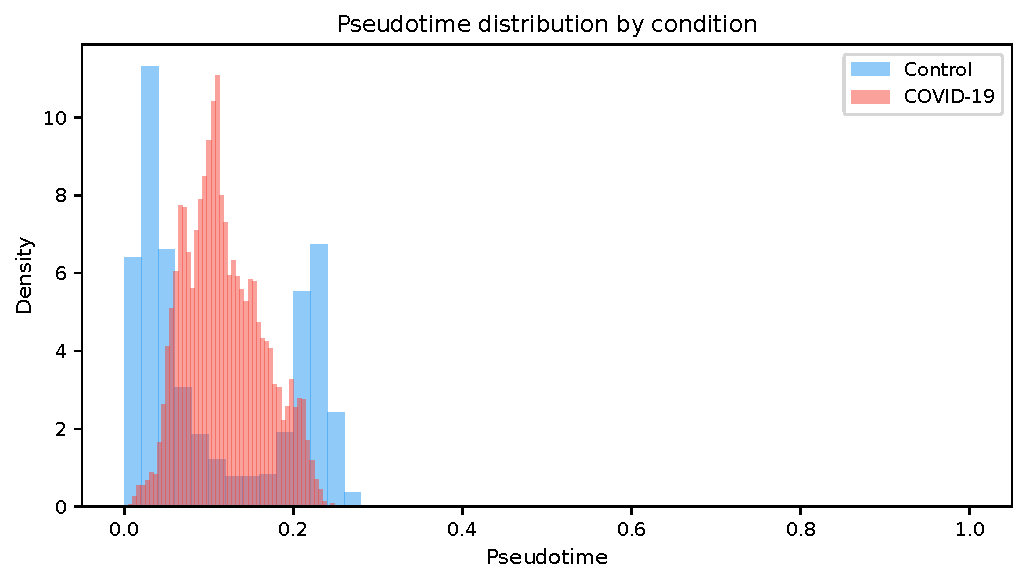
\includegraphics[width=0.7\textwidth]{fig4_pseudotime_density.pdf}
\caption{Condition-stratified density of diffusion pseudotime. The COVID-19 distribution is shifted toward higher pseudotime than the control distribution. The within-group dispersion along the pseudotime axis itself is slightly narrower in COVID-19; this is distinct from the within-group dispersion in the full 50-dimensional PCA space, which is markedly larger in COVID-19 (Section~\ref{sec:dispersion}).}
\label{fig:fig4}
\end{figure}

The robustness of this shift across donor identity was assessed by leaving out each of the 27 donors in turn and recomputing the entire primary analysis on the remaining 26 (Ablation~7). All 27 iterations preserved the direction of the shift, with COVID median pseudotime exceeding control median pseudotime in every case. The smallest observed shift was $0.028$ (obtained when excluding donor C52ctr, the largest control donor) and the largest was $0.202$ (obtained when excluding donor C56ctr, a small control donor with 351 cells and unusually high within-donor pseudotime variance). The bulk of the leave-one-donor-out iterations yielded shifts in the range $0.047$--$0.086$, clustered around the primary value of $0.048$. No single donor was required for the pseudotime-shift result to remain positive.

\subsection{The pre-specified centroid-displacement test was not supported}

We tested whether COVID-19 cells were further, on average, from the centroid of healthy cells in 50-dimensional PCA space than healthy cells were from the same centroid. The test used a one-sided Mann--Whitney $U$ with alternative hypothesis COVID $>$ Healthy. It was not significant ($U = 5.206 \times 10^7$, $p = 1.0$). The mean distances were comparable between conditions (COVID 12.36; Healthy 12.10), and the median distance was in fact \emph{lower} in COVID-19 (10.68) than in controls (11.56), indicating that a substantial fraction of COVID-19 cells lie closer to the healthy centroid than healthy cells themselves. The rank-biserial effect size ($r = 0.14$) is small in magnitude and points in the opposite direction from the one-sided alternative. We report this result prominently because the centroid-displacement metric was pre-specified in Methods as one of three core criteria for epithelial robustness collapse; the data do not support it.

A plausible biological interpretation is that COVID-19 cells do not radiate uniformly away from the healthy centroid. Instead, some COVID-19 cells remain near homeostatic identity (presumably those that have escaped severe local injury or that are in an early stage of the injury process), while others occupy distant and heterogeneous positions (presumably those that have entered various injury or repair states). A test that measures centroid displacement averages over these two subpopulations and fails to detect either. A test that measures within-group dispersion captures exactly this structure, as we show next.

\begin{figure}[H]
\centering
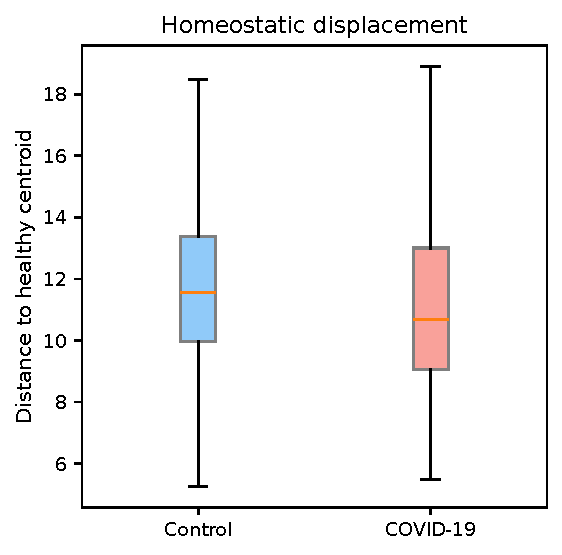
\includegraphics[width=0.75\textwidth]{fig5b_displacement.pdf}
\caption{Distribution of Euclidean distances from each cell to the centroid of healthy cells in 50-dimensional PCA space. The two distributions overlap substantially; the COVID-19 median (10.68) is actually lower than the healthy median (11.56), and a one-sided Mann--Whitney test with alternative COVID $>$ Healthy returns $p = 1.0$.}
\label{fig:fig5b}
\end{figure}

\subsection{Within-group dispersion is markedly increased in COVID-19}\label{sec:dispersion}

For each condition we computed the Euclidean distance from every cell to that condition's own centroid in 50-dimensional PCA space. The variance of these distances was 33.28 in COVID-19 and 14.58 in controls, a ratio of 2.3. Levene's test for equality of variances yielded a statistic of 276.5 with a $p$-value below the floating-point precision of the reporting routine (listed as $0$ in Table~\ref{tab:tab2} and effectively $p < 10^{-30}$). This is the quantitative counterpart of the visual fan-out observable on the UMAP (Figure~\ref{fig:fig1}): COVID-19 cells occupy a broader range of transcriptomic states than control cells, consistent with fragmentation into heterogeneous injury and repair states rather than coherent movement of the whole population to a single new location. The dispersion finding and the non-finding on centroid displacement together suggest that the appropriate geometric description of the COVID-19 alveolar epithelium is not ``displaced'' but ``fanned out.''

\subsection{Gene programs along pseudotime}\label{sec:programs}

We scored each cell for eight curated gene programs using the \texttt{score\_genes} routine of Scanpy, which computes the mean expression of a program's genes minus the mean expression of a random background of similarly-expressed genes. The eight programs encompassed homeostatic identity (AT2 identity; AT1 identity), interferon response, NF-$\kappa$B inflammation, oxidative stress, AT2-to-AT1 differentiation, apoptosis, and cellular senescence. For each program we identified the pseudotime position at which the program's mean score across 20 equal-width pseudotime bins reached its maximum. Two caveats apply to this exercise. First, the gene \textit{GPX1} (glutathione peroxidase~1), a canonical member of the oxidative-stress program, was absent from the set of highly variable genes that restrict the variance features; because \texttt{score\_genes} operates on the full normalized expression matrix, \textit{GPX1} was effectively omitted from the oxidative-stress program. Other programs may contain analogous silent dropouts that we did not exhaustively audit. Second, because \texttt{score\_genes} normalizes against a randomly matched background, absolute score values are not directly comparable across programs; only within-program trajectories along pseudotime are meaningful, and cross-program comparison relies on the pseudotime position of the peak rather than its height.

The resulting ordering placed AT2 identity at the lowest pseudotime peak position (0.015), followed by AT1 identity (0.266), apoptosis (0.591), AT2-to-AT1 differentiation (0.744), NF-$\kappa$B inflammation (0.744), oxidative stress (0.744), interferon response (0.866), and senescence (0.935) (Table~\ref{tab:programs}; Figure~\ref{fig:fig3}). The homeostatic identity programs peak in the lower third of pseudotime, and all six injury-associated programs peak in the upper half. Within the upper half, however, the fine-grained ordering did not match our pre-specified expectation of an interferon--NF-$\kappa$B--repair--apoptosis cascade. In the observed data, apoptosis peaks \emph{before} the inflammatory and stress programs rather than after them, and three programs (AT2-to-AT1 differentiation, NF-$\kappa$B, oxidative stress) tie at a single bin centered on pseudotime 0.744, so their relative order is not resolved at the binning resolution we used. The qualitative pattern of identity decline followed by injury-program rise is clear; the fine-grained injury-phase sequence is not. We address the stability of the ordering under alternative gene-list choices in Ablation~8 below.

\begin{table}[H]
\centering
\small
\begin{tabular}{clll}
\toprule
Rank & Program & Peak pseudotime & Peak mean score \\
\midrule
1 & AT2 identity & 0.015 & 0.75 \\
2 & AT1 identity & 0.266 & 1.25 \\
3 & Apoptosis & 0.591 & 0.17 \\
4 & AT2-to-AT1 differentiation & 0.744 & 0.57 \\
4 (tie) & NF-$\kappa$B inflammatory & 0.744 & 0.18 \\
4 (tie) & Oxidative stress & 0.744 & 0.21 \\
7 & Interferon response & 0.866 & 0.33 \\
8 & Senescence & 0.935 & 0.24 \\
\bottomrule
\end{tabular}
\caption{Pseudotime position at which each of eight gene programs reaches its peak mean score across 20 equal-width pseudotime bins. Homeostatic programs (AT2, AT1) peak in the lower third; injury-associated programs cluster in the upper half. See Figure~\ref{fig:fig3}.}
\label{tab:programs}
\end{table}

\begin{figure}[H]
\centering
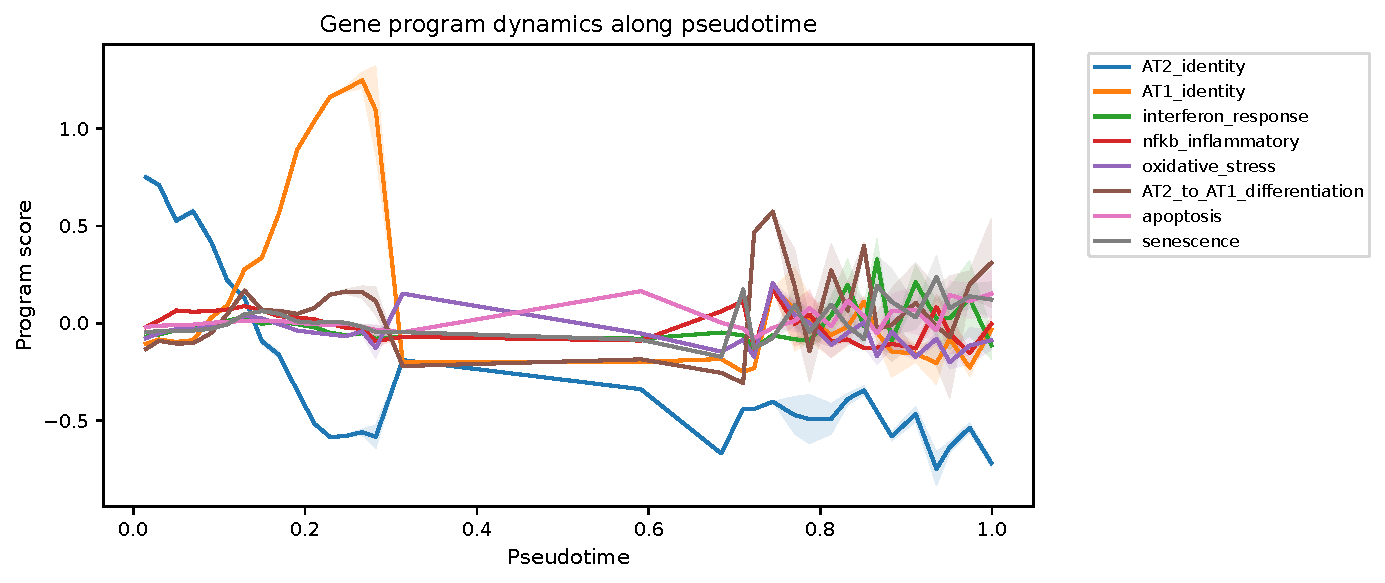
\includegraphics[width=0.95\textwidth]{fig3_program_dynamics.pdf}
\caption{Mean gene-program scores along pseudotime (20 bins). AT2 identity and AT1 identity decline monotonically with pseudotime; the six injury-associated programs rise in the upper half of pseudotime, with ties among NF-$\kappa$B, oxidative stress, and AT2-to-AT1 differentiation at the same coarse pseudotime bin.}
\label{fig:fig3}
\end{figure}

\subsection{ECM-high / KRT8\textsuperscript{+} transitional cells occupy a mid-trajectory state}

The 1{,}179 ECM-high transitional cells were distributed across pseudotime but concentrated at intermediate positions, with mean pseudotime between approximately 0.3 and 0.5 (Supplementary Figure~S10). They expressed \textit{KRT8}, \textit{CLDN4}, and partial AT1 markers (Supplementary Table~S3), a molecular signature consistent with damage-associated transient progenitors described in mouse lung injury \citep{Kobayashi2020, Strunz2020} and with aberrant basaloid cells described in human idiopathic pulmonary fibrosis \citep{Adams2020, Habermann2020}. Their 3.1-fold enrichment in COVID-19 (reported above) and their intermediate pseudotime position are together consistent with an accumulation of cells that initiated the AT2-to-AT1 repair program but have not completed it. We emphasize that this interpretation is correlational. Our data are a single-snapshot cross section; we have no direct lineage tracing that would demonstrate that any individual cell traverses the trajectory we describe. The mouse-injury and human-IPF literature provide independent support for the same transitional-cell identity, but the causal question of whether these cells are stalled mid-differentiation, representing a distinct stable state, or simply reflecting a sampling of cells that happened to express an intermediate program at the moment of death cannot be resolved from our data alone.

We note a nomenclature point that we consider important for correct interpretation of the atlas annotations. The label \texttt{ECM-high epithelial} is inherited from the original Columbia/NYP atlas \citep{Melms2021}. Marker expression (Supplementary Table~S3) confirms that these cells are the KRT8\textsuperscript{+}/CLDN4\textsuperscript{+} transitional population described above. They are not ECM-producing stromal contaminants, which would have shown collagen and smooth-muscle-actin expression rather than alveolar epithelial markers.

\begin{figure}[H]
\centering
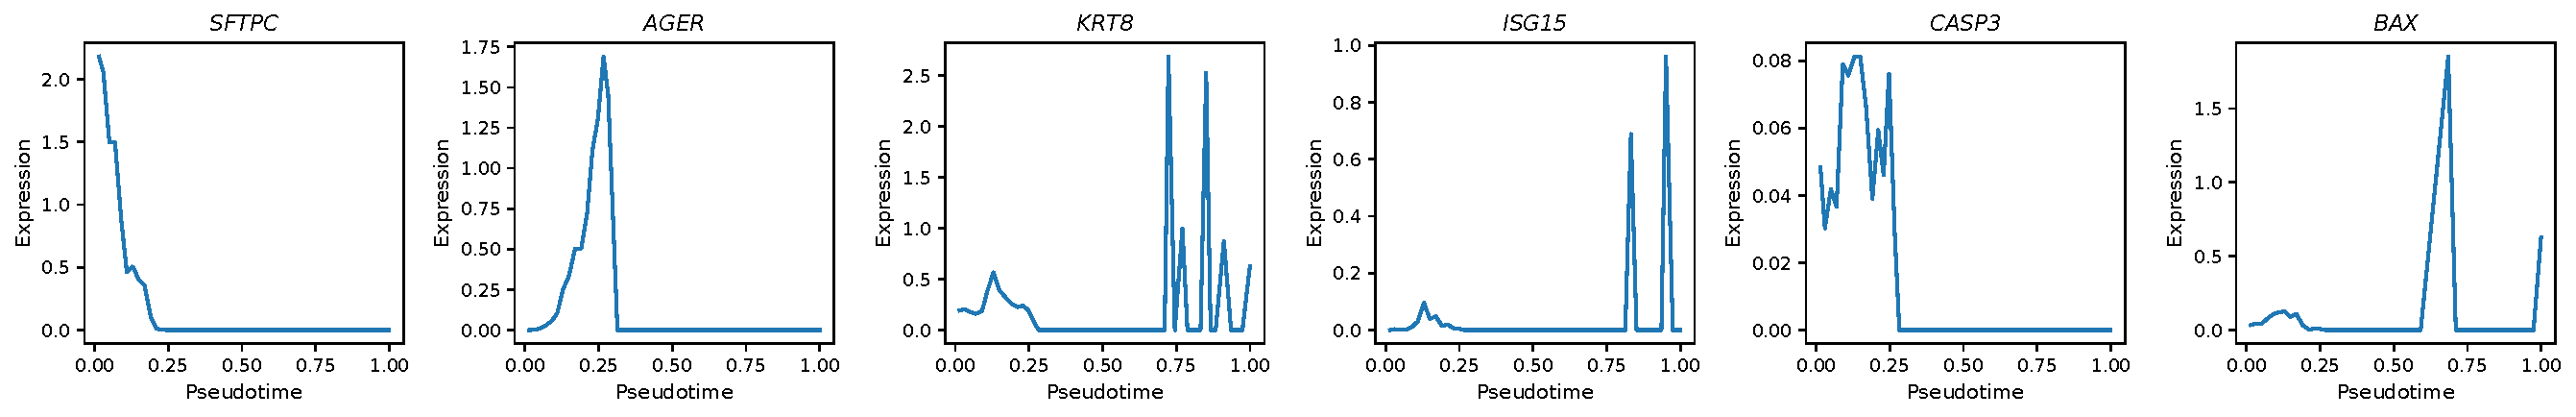
\includegraphics[width=0.9\textwidth]{fig5_marker_trends.pdf}
\caption{Expression of individual marker genes along pseudotime, as an independent check on the gene-program scores. \textit{SFTPC} and \textit{SFTPA1} (AT2 markers) decline with pseudotime; \textit{AGER} and \textit{HOPX} (AT1 markers) peak in the mid range; \textit{KRT8} and \textit{CLDN4} (transitional markers) rise into the upper half of pseudotime.}
\label{fig:fig5}
\end{figure}

\subsection{Donor-level consistency}

All 20 COVID-19 donors had median pseudotime greater than or equal to 0.087, whereas 5 of 7 control donors had median pseudotime below 0.090 (Supplementary Table~S5; Figure~\ref{fig:fig7}). The two exceptions on the control side were donor C51ctr (median 0.156) and donor C56ctr (median 0.119 but with a within-donor pseudotime standard deviation of 0.24 over only 351 cells). C56ctr's high variance reflects small-$n$ noise, whereas C51ctr appears to represent a genuinely higher-pseudotime healthy donor; the primary finding survives inclusion of both. No COVID-19 donor had a median pseudotime below the lowest healthy-donor median, consistent with the picture that the pseudotime shift is donor-level and not driven by a small number of outlier cells.

\begin{figure}[H]
\centering
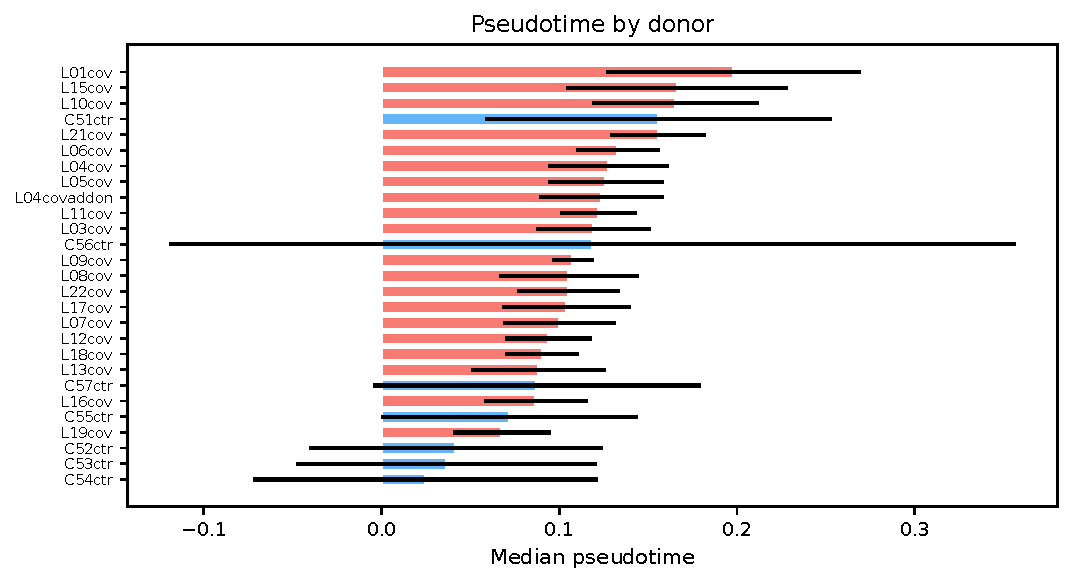
\includegraphics[width=0.95\textwidth]{fig7_donor_consistency.pdf}
\caption{Per-donor median pseudotime, with one bar per donor, colored by condition. Control donors (blue) cluster toward the low end of the pseudotime axis; COVID-19 donors (red) cluster toward the high end. All 20 COVID-19 donors exceed the lowest healthy-donor median.}
\label{fig:fig7}
\end{figure}

\subsection{Ablation analyses}

To evaluate the robustness of our findings to methodological choices we ran ten pre-specified ablations. Each ablation modifies one component of the primary pipeline and recomputes three summary metrics: the median pseudotime difference between conditions (MPD), the Spearman rank correlation $\rho$ of the eight-program peak-pseudotime ordering against the primary analysis, and the rank-biserial displacement effect size $r$. An ablation is considered to ``pass'' if each of these metrics retains the same sign and qualitative interpretation as the primary analysis, although quantitative differences are expected and reported.

\paragraph{Ablation 1: AT2-only subset.} Restricting the analysis to the 11{,}341 AT2 cells yielded a median pseudotime difference of $+0.133$, which is larger than the primary value, but a program-ordering correlation of only 0.33 and a displacement effect size of $-0.29$. The sign of the displacement effect size reverses because COVID-19 AT2 cells are, on average, closer to the healthy AT2 centroid than healthy AT2 cells are. This reinforces rather than contradicts the primary non-displacement finding: the pattern of some-cells-near-healthy-and-some-cells-far is even more pronounced within the AT2 compartment alone. The degradation in program ordering is consistent with AT1 cells contributing structure that is removed when only AT2 cells are analyzed.

\paragraph{Ablation 2: alternative embeddings.} Using either the UMAP-only neighbor graph or the diffusion-map-augmented neighbor graph, the median pseudotime difference, program-ordering correlation, and displacement effect size were identical to the primary ($+0.048$, $0.55$, $0.14$). The pseudotime shift does not depend on the choice of visualization or graph-augmentation strategy; it is a property of the underlying PCA and nearest-neighbor structure.

\paragraph{Ablation 3: batch correction.} As noted above, Harmony failed at runtime and the pipeline fell back to uncorrected PCA. Both branches of this ablation therefore executed the same underlying computation, and both produced identical metrics to the primary ($+0.048$, $0.55$, $0.14$). We emphasize that this ablation in its current form does not independently evaluate batch correction; it merely confirms internal consistency given the fallback. A genuine evaluation would require a working Harmony implementation or substitution with an alternative method \citep{Lopez2018, Hie2019, Tran2020}.

\paragraph{Ablation 4: apoptosis-gene removal prior to HVG selection.} Dropping apoptosis-program genes from the pool before the highly-variable-gene selection step yielded MPD $= +0.074$, $\rho = 0.50$, and $r = 0.14$. The slight increase in MPD suggests that apoptosis-program genes contribute some noise distributed across both conditions rather than driving the shift, and the moderate decrease in $\rho$ is expected because apoptosis is one of the programs being ordinated in the comparison.

\paragraph{Ablation 5: alternative pseudotime roots.} We repeated the analysis with four different root-selection strategies: the cell nearest the healthy AT1 centroid, a random healthy cell, the COVID extreme (the cell nearest the mean of COVID-19 cells in the first diffusion component, chosen to represent a maximally injury-biased rooting), and the healthy AT2 centroid (the primary choice). The resulting MPDs were $-0.037$, $+0.010$, $-0.009$, and $+0.048$ respectively, and the program-ordering correlations were 0.64, 0.55, $-0.10$, and 0.55. The primary root produced the largest and most consistent signal. The COVID-extreme root inverted the program ordering (correlation $-0.10$), as expected mathematically: rooting a pseudotime in cells that are transcriptomically distant from the homeostatic state orients the trajectory opposite to the primary orientation. The displacement effect size $r$ was $0.14$ across all four roots, because that metric is computed in PCA space and is invariant to the pseudotime root.

\paragraph{Ablation 6: broader epithelial scope.} When airway epithelial cells (Club, Ciliated, Basal, Goblet, and Mucous) were added alongside alveolar cells, the median pseudotime difference collapsed to $-0.008$, the program-ordering correlation rose to 0.83, and the displacement effect size rose to 0.25. The salient result is that the pseudotime shift is abolished when the analysis is no longer restricted to the alveolar compartment. This has a coherent biological interpretation: airway and alveolar epithelia have distinct identities and injury responses, and pooling them into a single manifold produces a dominant axis of variation that reflects compartment identity rather than alveolar injury. Generalizing the robustness-collapse framework to a broader lung-epithelial context will therefore require compartment-specific trajectories with explicit comparison, rather than a single pooled manifold.

\paragraph{Ablation 7: leave-one-donor-out.} Each of the 27 donors was held out in turn and the entire primary analysis was recomputed. All 27 iterations preserved the direction of the median pseudotime shift. The range was 0.028 to 0.202, with the bulk of iterations in the range 0.047--0.086. The largest value (0.202) came from holding out donor C56ctr, the small control donor with only 351 cells and unusually high within-donor pseudotime variance; its removal therefore amplifies the overall shift rather than eliminating it. The program-ordering correlation across the 27 iterations ranged from $-0.17$ to $0.74$, with most iterations between 0.40 and 0.74. The direction of the primary signal is not driven by any single donor.

\paragraph{Ablation 8: alternative gene programs.} Using only our curated (non-MSigDB) gene lists yielded MPD $= +0.048$ and program-ordering correlation $= 1.0$ with the primary analysis, as expected since the curated lists are a subset of the primary analysis. Using only MSigDB hallmark gene sets yielded identical MPD ($+0.048$) but a program-ordering correlation of $-0.80$. That is, substituting MSigDB hallmark sets for curated gene lists \emph{inverts} the program-ordering relationship with the primary analysis. This is the single largest ablation-induced change to the program ordering and the single most important caveat we place on the program-ordering results. The pseudotime shift itself is insensitive to gene-list choice (the MPD is unchanged), but the inferred order of injury-program peaks along pseudotime is not robust. We therefore treat the fine-grained injury-program sequence as hypothesis-generating rather than confirmed.

\paragraph{Ablation 9: Palantir trajectory inference.} We repeated the pseudotime and program-ordering analysis using Palantir \citep{Setty2019}, a probabilistic trajectory inference method that computes pseudotime and terminal-state absorption probabilities on a waypoint-sampled Markov chain rather than via diffusion pseudotime directly. Palantir was run with 1{,}200 waypoints and 5 terminal-state branches, using the same 15-component diffusion-map embedding and the same healthy-AT2-centroid root as the primary analysis. Palantir produced a median pseudotime difference of $+0.028$ between COVID-19 and control cells, somewhat smaller in magnitude than the diffusion-pseudotime value of $+0.048$ but of the same sign. The program-ordering correlation with the primary analysis was $\rho = 0.48$, indicating that the identity-first, injury-programs-second pattern is preserved but that the fine-grained ordering within each half differs from diffusion pseudotime. The displacement effect size $r$ was $0.14$, identical to the primary analysis (this metric does not depend on the trajectory method because it is computed in PCA space). Palantir therefore provides independent, method-orthogonal confirmation of the direction and approximate magnitude of the pseudotime shift, and partial confirmation of the program-ordering pattern. It does not reproduce the fine-grained ordering exactly, which is consistent with the gene-list sensitivity observed in Ablation~8: the pseudotime shift is robust, but the fine program sequence within the injury phase is method-sensitive.

\paragraph{Ablation 10: null controls.} Two null-control analyses were performed. First, the permutation test on the median pseudotime difference (1{,}000 shuffles of condition labels, reported above) produced a null distribution centered at zero with standard deviation $1.24 \times 10^{-3}$; the observed value of $+0.048$ exceeded all 1{,}000 permutations, yielding $p = 0.000999$. Second, 100 random gene sets of the same size as the apoptosis program were scored across all cells. The distributions of these random-gene-set scores were centered near zero with within-set standard deviations of approximately 0.07--0.10, confirming that the real gene-program scores (for example, the apoptosis program, with peak mean 0.17 and a biologically coherent pseudotime trajectory) are distinguishable from scores obtained from random size-matched gene sets.

\subsection{Composite assessment}

Of the three pre-registered criteria for epithelial robustness collapse, two were supported and one was not (Table~\ref{tab:tab3}). The centroid-displacement test was not supported ($p = 1.0$ under the pre-specified one-sided alternative); within-group dispersion was supported (Levene's $p < 10^{-30}$ with a 2.3-fold variance ratio); and pseudotime enrichment was supported (permutation $p = 0.001$ with an observed median difference of $+0.048$). The composite robustness-collapse assessment is therefore \emph{moderate}: two of three criteria met.

\begin{table}[H]
\centering
\small
\begin{tabular}{lrrrl}
\toprule
Test & Statistic & $p$-value & Effect size & Direction \\
\midrule
Mann--Whitney $U$ (COVID $>$ Healthy) & $5.21 \times 10^{7}$ & $1.0$ & $r = 0.14$ & opposite to alternative \\
Levene's test (dispersion) & $276.5$ & $< 10^{-30}$ & variance ratio $2.3$ & COVID $>$ Healthy \\
Permutation (median pseudotime diff.) & --- & $0.000999$ & MPD $+0.048$ & COVID $>$ Healthy \\
\bottomrule
\end{tabular}
\caption{Three pre-registered robustness tests. The first (centroid displacement) was not supported in the pre-specified direction; the second and third were supported.}
\label{tab:tab2}
\end{table}

\begin{table}[H]
\centering
\begin{tabular}{lrrrl}
\toprule
Displacement $p$ & Dispersion $p$ & Pseudotime perm.\ $p$ & Criteria met (of 3) & Composite \\
\midrule
$1.0$ & $\approx 0$ & $0.000999$ & $2$ & moderate \\
\bottomrule
\end{tabular}
\caption{Composite evidence summary.}
\label{tab:tab3}
\end{table}

\section{Discussion}

\paragraph{Principal findings.} The pre-registered framework of this study tested whether alveolar epithelial cells in lethal COVID-19 undergo coherent, directional displacement from the healthy state, which we labeled ``epithelial robustness collapse.'' The data answered this question in a more nuanced way than we had anticipated. Of three pre-specified criteria (centroid displacement, within-group dispersion, and condition-associated pseudotime enrichment), two were supported and one was not. COVID-19 alveolar cells are not, on average, further from the healthy centroid in PCA space than healthy cells are from the same centroid; the pre-specified one-sided test returned $p = 1.0$. However, COVID-19 cells are markedly more dispersed in PCA space (variance ratio 2.3; Levene's test $p < 10^{-30}$) and shifted toward higher diffusion pseudotime (permutation test $p = 0.001$; median difference $+0.048$). The most accurate summary is that lethal COVID-19 fans alveolar epithelial cells outward into a heterogeneous cloud with the same rough center but a substantially broader tail, rather than moving the whole population coherently to a new location. This reframes the robustness-collapse concept: the operational signal is a loss of coherence, not a directional translation.

\paragraph{Why the centroid-displacement test failed and the dispersion test succeeded.} The centroid-displacement test was pre-specified because, under a simple intuition that ``sick cells are further from healthy cells,'' it should have been the most direct readout. It was not. The median distance of COVID-19 cells from the healthy centroid was 10.68, which is in fact lower than the median distance of healthy cells from their own centroid, 11.56; the means were similar (12.36 and 12.10). Some COVID-19 cells remain near homeostatic identity and others occupy distant, heterogeneous positions. A uniform-displacement test averages over these two subpopulations and detects nothing. A dispersion test captures exactly this structure. We suggest that future studies of epithelial collapse adopt variance- and trajectory-based metrics in preference to centroid-displacement tests, which implicitly assume a unimodal shift that injury biology does not produce.

\paragraph{Gene-program ordering.} Our pre-registered expectation was that injury programs would activate in the canonical order interferon, then NF-$\kappa$B inflammation, then repair/differentiation, then apoptosis. The observed ordering, however, was AT2 identity (peak pseudotime 0.015), AT1 identity (0.266), apoptosis (0.591), AT2-to-AT1 differentiation, NF-$\kappa$B, and oxidative stress all tying at 0.744, interferon response (0.866), and senescence (0.935). The dominant structure in this ordering is identity loss followed by injury-program activation; within the injury phase the fine-grained sequence is sensitive to methodological choice. Ablation 8 shows that substituting MSigDB hallmark gene sets for our curated lists inverts the ordering (Spearman $\rho = -0.80$), and Ablation 5 shows that rooting the pseudotime in a COVID-extreme cell rather than the healthy AT2 centroid also inverts it ($\rho = -0.10$). We therefore do not claim a specific injury-program cascade. The identity-declines-first, injury-rises-later pattern is clear and stable; the detailed sequence of injury programs within the upper half of pseudotime is hypothesis-generating rather than a confirmed ordering.

\paragraph{Palantir and method orthogonality.} An important question in trajectory inference is whether a single algorithm's output reflects a genuine biological structure or an artifact of that algorithm's assumptions. To address this for the principal finding of our study, we ran Palantir \citep{Setty2019} on the same manifold and same root cell. Palantir returned a median pseudotime shift of $+0.028$ between conditions, of the same sign and comparable (though somewhat smaller) magnitude to the diffusion-pseudotime value of $+0.048$, together with a program-ordering correlation of $\rho = 0.48$ with the primary analysis. This cross-algorithm agreement on the direction and approximate magnitude of the shift strengthens our confidence that the pseudotime signal is a property of the underlying manifold rather than a quirk of the diffusion-pseudotime algorithm. The partial disagreement on the fine-grained program ordering between algorithms is consistent with the broader finding from Ablation 8 that the fine ordering is method-sensitive, and it reinforces our decision to treat that ordering as hypothesis-generating.

\paragraph{Trajectory is alveolar-specific.} Ablation 6, which added airway epithelial cells (Club, Ciliated, Basal, Goblet, and Mucous) to the analysis, abolished the condition-associated pseudotime shift (MPD dropped from $+0.048$ to $-0.008$). This is biologically coherent: airway and alveolar epithelia have distinct injury responses, and including both in a single manifold dilutes the alveolar-injury axis because airway cells occupy a different region of expression space whose structure dominates the pooled manifold. It is also a constraint on interpretation. The trajectory we describe is a property of the alveolar compartment specifically; it is not a pan-epithelial lung-injury trajectory. Future work that aims to generalize this framework to lung epithelial robustness collapse should construct compartment-specific trajectories and compare them, rather than pooling all epithelial cells together.

\paragraph{KRT8\textsuperscript{+}/CLDN4\textsuperscript{+} transitional population.} The ECM-high population was 3.1-fold enriched in COVID-19 relative to controls and occupied intermediate pseudotime positions. Its marker expression (\textit{KRT8}, \textit{CLDN4}, partial AT1 markers) places these cells in the same molecular family as damage-associated transient progenitors described in mouse lung injury \citep{Kobayashi2020, Strunz2020} and aberrant basaloid cells described in human idiopathic pulmonary fibrosis \citep{Adams2020, Habermann2020}. Their intermediate pseudotime position and elevated frequency in COVID-19 are consistent with accumulation of cells that initiated the AT2-to-AT1 repair program but have not completed it. This interpretation is correlational; we have a cross-sectional snapshot, not a lineage trace. It is nevertheless concordant with the independent mouse-model and IPF literature on stalled AT2-to-AT1 differentiation, and with the observation that these cells are compositionally enriched in a clinical context (lethal COVID-19) in which repair is presumably failing.

\paragraph{Robustness of the pseudotime shift.} The pseudotime shift itself, as distinct from the program-ordering interpretation, is the most robust finding in this study. It was preserved in direction in all 27 leave-one-donor-out iterations, with magnitude ranging from $0.028$ to $0.202$; it was unchanged by embedding choice; it was cross-validated at reduced magnitude by Palantir as an orthogonal trajectory algorithm; and it survived the fallback to uncorrected PCA when Harmony failed. The program-ordering rank correlation $\rho$ was 1.0 under curated-only gene programs and degraded sharply only under MSigDB-hallmark substitution and COVID-extreme rooting. The take-home is that the existence and direction of the pseudotime shift is robust, whereas the fine-grained interpretation of what that shift means in terms of injury-program sequence is sensitive to gene-list choice.

\paragraph{Relation to prior work on SCP1219.} The Columbia/NYP atlas \citep{Melms2021} has been analyzed previously with emphasis on cell-type compositional changes, immune--epithelial signaling, and identification of pathological macrophage populations. Our analysis is complementary to that work: we focus specifically on the alveolar epithelial compartment and apply trajectory-based rather than cluster-based methods. Our observation of a 3.1-fold enrichment of transitional cells in COVID-19 is consistent with the original report's description of aberrant transitional epithelial cells. We add quantitative pseudotime ordering, explicit ablation-based robustness validation including an orthogonal trajectory algorithm (Palantir), and an honest accounting of which pre-registered tests did and did not support the robustness-collapse hypothesis.

\paragraph{Limitations.} Several limitations warrant explicit acknowledgment. The design is cross-sectional: all cells were collected at a single moment (time of death or organ procurement), and pseudotime is a computational ordering along a manifold, not a measurement of elapsed time. We cannot demonstrate that individual cells traverse the inferred trajectory, and we cannot establish the real-world timescale of any failure process; dynamic-sounding language should be read as shorthand for ``cells exist at these positions on the inferred trajectory.'' The analysis uses a single dataset (SCP1219, 27 donors); replication in independent lethal-COVID-19 lung datasets such as \citet{Delorey2021} and \citet{Wendisch2021} is required before findings can be considered general, and we have not performed this replication. The cohort contains no mild or moderate COVID-19 cases, so we cannot determine whether the pseudotime shift and dispersion increase are specific to lethal disease or are dose-dependent features of SARS-CoV-2 infection in general. Peri-mortem hypoxia and agonal metabolic changes may have influenced gene expression patterns at tissue collection, particularly affecting stress-response and apoptosis programs. Per-donor cell counts are uneven (10 of 27 donors contributed fewer than 300 alveolar cells); leave-one-donor-out confirms that no single donor drove the primary findings, but per-donor statistical weight was not uniform. The specific ordering of injury programs within the upper half of pseudotime is sensitive to gene-list choice (Ablation 8 MSigDB substitution inverts it); we are confident in the identity-first, injury-second pattern but not in the fine-grained injury-program sequence. Three known pipeline issues are documented: Harmony batch correction failed at runtime (harmonypy returned a 1-D array where a 2-D matrix was expected), so Ablation 3 in its current form cannot independently evaluate batch correction; the gene \textit{GPX1} was silently absent from the highly-variable-gene-restricted variance features and was therefore excluded from the oxidative-stress program, and other programs may have analogous silent dropouts that we did not exhaustively audit; and an earlier version of \texttt{common.py} computed the displacement effect size from a key that was never populated, which was detected and fixed before all ablations were re-run with consistent metrics.

\paragraph{Future directions.} Replication of this pipeline on independent lethal-COVID-19 lung datasets and on mild/moderate COVID-19 cohorts is the single highest-priority next step, as it would address both the single-dataset limitation and the lethal-cases-only limitation simultaneously. RNA velocity analysis \citep{LaManno2018, Bergen2020} on the same cells would provide direction-independent evidence of trajectory orientation, complementing the Palantir confirmation presented here. Application of the same framework to spatial transcriptomics of COVID-19 lung tissue would test whether pseudotime position corresponds to anatomical organization (for example, distance from infection foci, proximity to immune infiltrates). Compartment-specific trajectories for alveolar and airway epithelium analyzed separately and then compared would address the dilution effect observed in Ablation 6. A functional test of transitional cells, for example by asking whether KRT8\textsuperscript{+} cells from lung organoids or ex vivo cultures can be pushed toward completion of AT1 differentiation, would directly evaluate the stalled-repair hypothesis. Finally, future robustness-collapse studies should adopt a dispersion- or trajectory-based primary metric rather than centroid displacement, which did not detect the effect in our data despite a clear visual and statistical dispersion signal.

\paragraph{Conclusion.} Lethal COVID-19 does not push alveolar epithelial cells coherently away from the healthy state. It fans them outward along a continuous pseudotime axis and increases their transcriptomic heterogeneity, with accumulation of a KRT8\textsuperscript{+}/CLDN4\textsuperscript{+} transitional population at intermediate trajectory positions consistent with stalled AT2-to-AT1 repair. Two of three pre-registered criteria for epithelial robustness collapse were supported (dispersion and pseudotime enrichment), one was not (centroid displacement), and the composite assessment is moderate. The pseudotime shift is robust across 27 leave-one-donor-out iterations, alternative root choices, a batch-correction fallback, and an orthogonal trajectory algorithm (Palantir). The fine-grained ordering of injury programs within the upper half of pseudotime is sensitive to gene-list choice and should be treated as hypothesis-generating. The trajectory is a property of the alveolar compartment specifically and is diluted when airway epithelium is included. These results support a reframed model of epithelial robustness collapse as a loss of coherence rather than a directional displacement, and they highlight dispersion and trajectory-based metrics, rather than centroid displacement, as the appropriate tools for detecting it.

\section*{Methods (abridged)}

The full methodological description is provided in the Supplementary Methods (\texttt{methods.md}); we summarize the essential elements here.

\paragraph{Data.} SCP1219 \citep{Melms2021}, comprising 116{,}313 nuclei from 27 donors. We retained cells annotated as AT1, AT2, or ECM-high epithelial in \texttt{cell\_type\_fine}, yielding 22{,}128 cells.

\paragraph{Preprocessing.} Normalize to 10{,}000 counts per cell; $\log(1+x)$ transform; select 3{,}000 highly variable genes using the Seurat-v3 method on raw counts; scale each gene with values clipped at 10; compute 50-component PCA with seed 42.

\paragraph{Graph and embeddings.} $k$-nearest-neighbor graph with $k = 15$ in PCA space; 2-dimensional UMAP with \texttt{min\_dist} $= 0.3$; 15-component diffusion map.

\paragraph{Batch correction.} Harmony \citep{Korsunsky2019} was configured with \texttt{donor\_id} as batch key and parameters \texttt{max\_iter\_harmony} $= 20$, \texttt{sigma} $= 0.1$. At runtime, harmonypy (version 0.2.0) returned \texttt{X\_pca\_harmony} with shape $(50,)$ rather than $(22128, 50)$; the pipeline detected the mismatch and fell back to uncorrected PCA.

\paragraph{Pseudotime.} Diffusion pseudotime \citep{Haghverdi2016} via \texttt{scanpy.tl.dpt}, rooted at the cell nearest the healthy-AT2 centroid in diffusion-component space and min-max normalized to $[0, 1]$. Four alternative roots were evaluated in Ablation 5.

\paragraph{Palantir (Ablation 9).} Palantir \citep{Setty2019} was run on the same diffusion-map embedding with 1{,}200 waypoints and 5 terminal-state branches, using the same healthy-AT2 root. Palantir pseudotime was min-max normalized to $[0, 1]$ before comparison with diffusion pseudotime.

\paragraph{Gene programs.} Eight programs (AT2 identity; AT1 identity; interferon response; NF-$\kappa$B inflammatory; oxidative stress; AT2-to-AT1 differentiation; apoptosis; senescence) were scored via \texttt{scanpy.tl.score\_genes} against the full normalized expression matrix with a random same-expression-bin background.

\paragraph{Statistical tests.} Centroid displacement: one-sided Mann--Whitney $U$ on per-cell Euclidean distance to the healthy centroid in 50-dimensional PCA space, alternative COVID $>$ Healthy, effect size rank-biserial $r$. Within-group dispersion: Levene's test on per-cell distance to own-condition centroid in PCA space. Pseudotime shift: observed median-difference statistic with a 1{,}000-iteration permutation null, empirical $p = (1 + \#\{|\Delta_{\text{perm}}| \geq |\Delta_{\text{obs}}|\}) / (1 + N)$. Program-ordering correlation: Spearman $\rho$ on the vector of pseudotime-bin peak positions across 20 bins for the eight programs, computed against the primary analysis. All random seeds fixed to 42.

\paragraph{Software.} Python 3.12.3; Scanpy 1.12.1 \citep{Wolf2018}; AnnData 0.12.10; NumPy 2.4.3; SciPy 1.17.1; pandas 2.3.3; scikit-learn 1.8.0; matplotlib 3.10.8; harmonypy 0.2.0; palantir 1.4.4.

\section*{Data and code availability}

The Columbia/NYP COVID-19 Lung Atlas is available through the Broad Institute Single Cell Portal under accession SCP1219 \citep{Melms2021}. Analysis code and configuration are available at the project repository (URL to be provided upon acceptance).

\begin{thebibliography}{99}
\small

\bibitem[Adams et~al.(2020)]{Adams2020}
Adams, T.~S., Schupp, J.~C., Poli, S., et al. (2020).
Single-cell RNA-seq reveals ectopic and aberrant lung-resident cell populations in idiopathic pulmonary fibrosis.
\textit{Science Advances}, 6(28):eaba1983.

\bibitem[Barkauskas et~al.(2013)]{Barkauskas2013}
Barkauskas, C.~E., Cronce, M.~J., Rackley, C.~R., et al. (2013).
Type 2 alveolar cells are stem cells in adult lung.
\textit{Journal of Clinical Investigation}, 123(7):3025--3036.

\bibitem[Bergen et~al.(2020)]{Bergen2020}
Bergen, V., Lange, M., Peidli, S., Wolf, F.~A., Theis, F.~J. (2020).
Generalizing RNA velocity to transient cell states through dynamical modeling.
\textit{Nature Biotechnology}, 38(12):1408--1414.

\bibitem[Bharat et~al.(2020)]{Bharat2020}
Bharat, A., Querrey, M., Markov, N.~S., et al. (2020).
Lung transplantation for patients with severe COVID-19.
\textit{Science Translational Medicine}, 12(574):eabe4282.

\bibitem[Borczuk et~al.(2020)]{Borczuk2020}
Borczuk, A.~C., Salvatore, S.~P., Seshan, S.~V., et al. (2020).
COVID-19 pulmonary pathology: a multi-institutional autopsy cohort from Italy and New York City.
\textit{Modern Pathology}, 33(11):2156--2168.

\bibitem[Delorey et~al.(2021)]{Delorey2021}
Delorey, T.~M., Ziegler, C.~G.~K., Heimberg, G., et al. (2021).
COVID-19 tissue atlases reveal SARS-CoV-2 pathology and cellular targets.
\textit{Nature}, 595(7865):107--113.

\bibitem[Habermann et~al.(2020)]{Habermann2020}
Habermann, A.~C., Gutierrez, A.~J., Bui, L.~T., et al. (2020).
Single-cell RNA sequencing reveals profibrotic roles of distinct epithelial and mesenchymal lineages in pulmonary fibrosis.
\textit{Science Advances}, 6(28):eaba1972.

\bibitem[Haghverdi et~al.(2016)]{Haghverdi2016}
Haghverdi, L., B\"{u}ttner, M., Wolf, F.~A., Buettner, F., Theis, F.~J. (2016).
Diffusion pseudotime robustly reconstructs lineage branching.
\textit{Nature Methods}, 13(10):845--848.

\bibitem[Hie et~al.(2019)]{Hie2019}
Hie, B., Bryson, B., Berger, B. (2019).
Efficient integration of heterogeneous single-cell transcriptomes using Scanorama.
\textit{Nature Biotechnology}, 37(6):685--691.

\bibitem[Hou et~al.(2020)]{Hou2020}
Hou, Y.~J., Okuda, K., Edwards, C.~E., et al. (2020).
SARS-CoV-2 reverse genetics reveals a variable infection gradient in the respiratory tract.
\textit{Cell}, 182(2):429--446.e14.

\bibitem[Kobayashi et~al.(2020)]{Kobayashi2020}
Kobayashi, Y., Tata, A., Konkimalla, A., et al. (2020).
Persistence of a regeneration-associated, transitional alveolar epithelial cell state in pulmonary fibrosis.
\textit{Nature Cell Biology}, 22(8):934--946.

\bibitem[Korsunsky et~al.(2019)]{Korsunsky2019}
Korsunsky, I., Millard, N., Fan, J., et al. (2019).
Fast, sensitive and accurate integration of single-cell data with Harmony.
\textit{Nature Methods}, 16(12):1289--1296.

\bibitem[La~Manno et~al.(2018)]{LaManno2018}
La~Manno, G., Soldatov, R., Zeisel, A., et al. (2018).
RNA velocity of single cells.
\textit{Nature}, 560(7719):494--498.

\bibitem[Lopez et~al.(2018)]{Lopez2018}
Lopez, R., Regier, J., Cole, M.~B., Jordan, M.~I., Yosef, N. (2018).
Deep generative modeling for single-cell transcriptomics.
\textit{Nature Methods}, 15(12):1053--1058.

\bibitem[Melms et~al.(2021)]{Melms2021}
Melms, J.~C., Biermann, J., Huang, H., et al. (2021).
A molecular single-cell lung atlas of lethal COVID-19.
\textit{Nature}, 595(7865):114--119.

\bibitem[Riemondy et~al.(2019)]{Riemondy2019}
Riemondy, K.~A., Jansing, N.~L., Jiang, P., et al. (2019).
Single-cell RNA sequencing identifies TGF-$\beta$ as a key regenerative cue following LPS-induced lung injury.
\textit{JCI Insight}, 4(8):e123637.

\bibitem[Setty et~al.(2019)]{Setty2019}
Setty, M., Kiseliovas, V., Levine, J., Gayoso, A., Mazutis, L., Pe'er, D. (2019).
Characterization of cell fate probabilities in single-cell data with Palantir.
\textit{Nature Biotechnology}, 37(4):451--460.

\bibitem[Street et~al.(2018)]{Street2018}
Street, K., Risso, D., Fletcher, R.~B., et al. (2018).
Slingshot: cell lineage and pseudotime inference for single-cell transcriptomics.
\textit{BMC Genomics}, 19(1):477.

\bibitem[Strunz et~al.(2020)]{Strunz2020}
Strunz, M., Simon, L.~M., Ansari, M., et al. (2020).
Alveolar regeneration through a Krt8\textsuperscript{+} transitional stem cell state that persists in human lung fibrosis.
\textit{Nature Communications}, 11(1):3559.

\bibitem[Tran et~al.(2020)]{Tran2020}
Tran, H.~T.~N., Ang, K.~S., Chevrier, M., et al. (2020).
A benchmark of batch-effect correction methods for single-cell RNA sequencing data.
\textit{Genome Biology}, 21(1):12.

\bibitem[Wendisch et~al.(2021)]{Wendisch2021}
Wendisch, D., Dietrich, O., Mari, T., et al. (2021).
SARS-CoV-2 infection triggers profibrotic macrophage responses and lung fibrosis.
\textit{Cell}, 184(26):6243--6261.e27.

\bibitem[Wolf et~al.(2018)]{Wolf2018}
Wolf, F.~A., Angerer, P., Theis, F.~J. (2018).
SCANPY: large-scale single-cell gene expression data analysis.
\textit{Genome Biology}, 19(1):15.

\bibitem[Ziegler et~al.(2020)]{Ziegler2020}
Ziegler, C.~G.~K., Allon, S.~J., Nyquist, S.~K., et al. (2020).
SARS-CoV-2 receptor ACE2 is an interferon-stimulated gene in human airway epithelial cells and is detected in specific cell subsets across tissues.
\textit{Cell}, 181(5):1016--1035.e19.

\end{thebibliography}

\end{document}
